\documentclass[xcolor=dvipsnames]{beamer}
\usepackage{amsmath}
\usepackage{amssymb}
\usepackage[english]{babel}
\usepackage[latin1]{inputenc}
\usepackage{times}
\usepackage[T1]{fontenc}
\usepackage{graphicx}
\usepackage[absolute, overlay]{textpos}
\usepackage{tikz}
\usepackage{multimedia}
\usepackage{soul}
\usepackage{hyperref}
\usepackage{wasysym}
\usepackage{cancel}
\def\urltilda{\kern -.15em\lower .7ex\hbox{\~{}}\kern .04em}
\def\deg{^{\circ}}

\setlength{\TPHorizModule}{0.01\textwidth}
\setlength{\TPVertModule}{\TPHorizModule}

\definecolor{darkyellow}{rgb}{1,0.75,0}
\definecolor{black}{rgb}{0,0,0}
\definecolor{orange}{rgb}{0.9, 0.5, 0.0}

\mode<presentation>
{
  \usetheme{Warsaw}
  \usecolortheme[named=darkyellow]{structure}	
  \setbeamercovered{transparent}
  \setbeamercolor{item}{fg=black}
}

%\beamerdefaultoverlayspecification{<+->}

\newcommand{\vect}[1]{\boldsymbol{#1}}
\newcommand{\params}{\Xi}
\newcommand{\Eobsi}{E'_i}
\newcommand{\phiobsi}{\phi'_i}
\newcommand{\Etruei}{E_i}
\newcommand{\phitruei}{\phi_{i}}
\newcommand{\Eobsij}{E'_{ij}}
\newcommand{\phiobsij}{\phi'_{ij}}
\newcommand{\Etrueij}{E_{ij}}
\newcommand{\phitrueij}{\phi_{ij}}
\newcommand{\obs}{\mathrm{obs}}
\newcommand{\true}{\mathrm{true}}
\newcommand{\Like}{\mathcal{L}}
\newcommand{\ntot}{{n_\mathrm{tot}}}
\newcommand{\ntotj}{{n_{\mathrm{tot},j}}}
\newcommand{\diff}{\mathrm{d}}
\newcommand{\cblue}[1]{{\color[rgb]{0.1, 0.0, 0.6} #1}}
\newcommand{\cgreen}[1]{{\color[rgb]{0.0, 0.6, 0.1} #1}}
\newcommand{\corange}[1]{{\color[rgb]{0.9, 0.5, 0.0} #1}}
\newcommand{\cbluewhen}[2]{{\color#2[rgb]{0.1, 0.0, 0.6} #1}}
\newcommand{\cgreenwhen}[2]{{\color#2[rgb]{0.0, 0.6, 0.1} #1}}
\newcommand{\corangewhen}[2]{{\color#2[rgb]{0.9, 0.5, 0.0} #1}}
\newcommand{\vrel}{v_{\mathrm{rel}}}
\newcommand{\mn}{m_{\rm nuc}}
\newcommand{\mx}{m_\chi}
\newcommand{\nc}{\newcommand}
\nc{\x}{{\bf x }}
\nc{\kk}{{\bf k }}
\nc{\f}{{\bf f }}
\nc{\e}{{\bf e }}
\nc{\gag}{g_{a \gamma}}
\nc{\ud}{\mathrm{d}}
\nc{\igev}{GeV$^{-1}$}
\nc{\ssi}{\sigma_{\mathrm{SI}}}
\nc{\ssd}{\sigma_{\mathrm{SD}}}
\nc{\tq}{\tilde \q}
\nc{\qmin}{q_{\mathrm{min}}}
\nc{\qmax}{q_{\mathrm{max}}}
\nc{\dmin}{\delta_{\mathrm{min}}}
\nc{\dmax}{\delta_{\mathrm{max}}}
\nc{\ie}{i.e.\xspace}
\nc{\del}{\partial}
\nc{\Cin}{C_{\mathrm{in}}}
\nc{\Cout}{C_{\mathrm{out}}}
\nc{\shat}{\hat \sigma}
\nc{\ket}[1]{| #1 \rangle}
\nc{\bra}[1]{\langle #1 |}
\nc{\braket}[2]{\langle #1 | #2 \rangle}
\nc{\speclarrow}{$\boldsymbol{\rightarrow}$\ }
\nc{\bi}{\begin{itemize}}
\nc{\ei}{\end{itemize}}
\nc{\bfr}[1]{\begin{frame}\frametitle{#1}}

\AtBeginSection[]
{
  \begin{frame}<beamer>
    \frametitle{Outline of Lecture 1}
  \begin{columns}[t]
	\column{0.8\textwidth}
	\tableofcontents[sections={1},currentsection,subsections]
        \vspace{3mm}
	\tableofcontents[sections={2},currentsection,subsections]
        \vspace{3mm}
	\tableofcontents[sections={3},currentsection,subsections]
  \end{columns}	
  \end{frame}
}

\setbeamertemplate{subsection in head/foot shaded}
{\textcolor{structure!80!black}{\insertsubsectionhead}}
\setbeamertemplate{subsection in head/foot}{\textcolor{black}\insertsubsectionhead}

\title[{\color[rgb]{0, 0, 0}Astroparticle Phenomenology I: Cosmology}]{\textcolor{black}{Lectures in Astroparticle Phenomenology\\ I. Particle Cosmology}}
\author[Pat Scott -- Feb 25 -- University of Sydney]{Pat Scott}
\institute{\small{McGill University / Imperial College London}}
\date[Feb 25, 2014]{Slides available from \color[rgb]{0.1, 0.0, 0.6} \href{http://www.physics.mcgill.ca/~patscott}{\tt www.physics.mcgill.ca/{\urltilda}patscott}}
\subject{Talks}
\pgfdeclareimage[height=1cm]{university-logo}{McGill_crest}
\logo{\pgfuseimage{university-logo}}

\begin{document}

\maketitle


\begin{frame}
  \frametitle{Lecture Plan}

  \cblue{Today}: Particle Cosmology
  \begin{itemize}
    \item $\Lambda$CDM
    \item Power spectra of cosmological perturbations
    \item Reheating, Big Bang nucleosynthesis, cosmic strings
  \end{itemize}
  \vspace{3mm}

  \cblue{Tomorrow} (SIfA Redfern):  Dark Matter
  \begin{itemize}
    \item Theories
    \item Production
    \item Direct + indirect detection
  \end{itemize}
  \vspace{3mm}

  \cblue{Thursday} (back here again):  Global Fits
  \begin{itemize}
    \item Techniques, status and coming developments
  \end{itemize}
    
\end{frame}


\begin{frame}
  \frametitle{Other cool stuff I won't be covering directly}
    (but that we can chat about at the end of one of lectures if you like)\vspace{1cm}

  \begin{itemize}
    \item Neutrino mass models / GUTs and their observables 
    \item Cosmic ray production + propagation
    \item Baryogenesis / leptogenesis
    \item Reionisation
  \end{itemize}\vspace{3cm}

\end{frame}


\begin{frame}
  \frametitle{Outline of Lecture 1}
  \begin{columns}[t]
	\column{0.8\textwidth}
	\tableofcontents[sections={1}]
        \vspace{3mm}
	\tableofcontents[sections={2}]
        \vspace{3mm}
	\tableofcontents[sections={3}]
  \end{columns}	
\end{frame}

\section{Cosmological Models}

\subsection{General}

\begin{frame}
  \frametitle{Setting up a framework for cosmology}

  \visible<1->{
    \alert{Step 1.}\\
    Assume the Universe to be isotropic and homogeneous\\$\implies$ Friedmann-Robertson Walker (FRW) metric:
    \begin{equation}
      g_{\mu\nu}x^\mu x^\nu = \mathsf{d}t^2 + R(t)^2\left(\frac{\mathsf{d}r^2}{1-kr^2} +r^2\mathsf{d}\Omega^2\right).
    \end{equation}
  }
  \begin{itemize}
    \item This is our distance measure in spacetime.  
    \item Everything but $R(t)$ is determined by isotropy \& homogeneity.
  \end{itemize}

  \vspace{3mm}
  \visible<2->{
  \alert{Step 2.}\\
  Take the Einstein Field Equations from General Relativity:
  \begin{equation}
    \label{EFE}
    \alert<3->{\visible<3->{\mathsf{geometry}}\hspace{10mm}G_{\mu\nu}} = 8\pi G \alert<4->{T_{\mu\nu} - \Lambda} g_{\mu\nu}.\hspace{5mm}\alert{\visible<4->{\mathsf{energy}}}
  \end{equation}}
  \visible<5->{$\rightarrow$ Tells us how geometry of space adjusts to mass/energy}

  \begin{textblock}{100}(37, 75.5)
    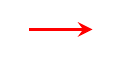
\begin{tikzpicture}[line width=1.3pt, color=red]
      \draw<3->[-stealth] (0,0) -- (0.8,0);
    \end{tikzpicture}
  \end{textblock}

  \begin{textblock}{100}(67, 70)
    
\begin{tikzpicture}[line width=1.3pt, color=red]
      \draw<4->[-stealth] (2,0) .. controls (1,0.5) .. (0,0);
    \end{tikzpicture}
  \end{textblock}

\end{frame}

\begin{frame}
  \frametitle{Setting up a framework for cosmology}

  \visible<1->{
  \alert{Step 3.}\\
  Solve $\mu=0,\nu=0$ of Einstein Eq. $\implies$ \alert<3>{\textit{Friedmann Equation}}:
  \begin{equation}
    \footnotesize
    \alert<3>{H(t)^2\equiv \left(\frac{\dot{R}(t)}{R(t)}\right)^2 = \frac{8\pi G}{3}\rho(t) - \frac{k}{R(t)^2}.}
  \end{equation}}
  \visible<2->{Solving this gives Hubble parameter $H(t)$ for some
  \begin{itemize}
    \item relationship between energy density and the scalefactor $R(t) = f[\rho(t)]$
    \item curvature $k\in\{+1,0,-1\}$
  \end{itemize}}
  \visible<3->{\alert<3>{$H(t)$ encodes the dynamic evolution of the Universe}}

  \vspace{4mm}
  \visible<4->{
  \textbf{Critical density:}
  
  For a flat Universe $k=0$. This defines 
  \[ \begin{array}{lrcl}
    \mathsf{\textit{critical density: }}  &\rho_\mathsf{c} &=& \frac{3H(t)}{8\pi G}\vspace{0.8mm}\\
    \mathsf{\textit{cosmological density: }} &\Omega_x &\equiv& \frac{\rho_x}{\rho_c}
  \end{array} \] 
  }

\end{frame}

\begin{frame}
  \frametitle{Equations of state}

  \textbf{Equations of state:}

  1st law of thermodynamics ($\mu=0$ in conservation of $T_{\mu\nu}$) is
  \begin{equation}
    \mathsf{d}(\rho R^3) = -p\mathsf{d}(R^3), \hspace{5mm}\mathsf{i.e.}\ \Delta E = -p\Delta V
  \end{equation}
  with a constant equation of state $\rho = wp$, we get energy density-scalefactor relations 
  \begin{equation}
    \rho \varpropto R^{-3(1+w)}
  \end{equation}
  For different types of energy:
  $\begin{array}{llcl}
  \mathsf{\textbf{\color[rgb]{0.1, 0.0, 0.6}Matter:}} &w=0 &\implies& \rho \varpropto R^{-3}\\
  \mathsf{\textbf{\color[rgb]{0.1, 0.0, 0.6}Radiation:}} &w=1/3 &\implies& \rho \varpropto R^{-4}\\
  \mathsf{\textbf{\color[rgb]{0.1, 0.0, 0.6}Vacuum ($\Lambda$):}} &w=-1 &\implies& \rho \varpropto constant
  \end{array}$

  \vspace{3mm}This is basically enough to solve the Friedmann Equation.

\end{frame}

\subsection{$\Lambda$CDM}

\begin{frame}
  \frametitle{Ingredients of $\Lambda$CDM}

  $\begin{array}{ll}  
  {\sf \textbf{Ingredients\ required}} & {\sf \textbf{Choices\ in\ }}\boldsymbol\Lambda{\sf \textbf{CDM}} \\
  {\sf \textbf{for\ a\ cosmological\ model}} &  \vspace{2mm}\\
  {\sf A\ theory\ of\ gravity} & {\sf GR}  \\
  {\sf +\ associated\ assumptions} & + {\sf isotropy, homogeneity} \vspace{2mm}\\ 
  {\sf Types\ of\ energy} & {\sf radiation, \alert<2>{matter}, vacuum/dark\ energy} \vspace{2mm}\\
  {\sf their\ equations\ of\ state} & \alert<2>{w =} 1/3,\ \alert<2>{0},\ -1/{\sf other} \vspace{2mm}\\
  {\sf \alert<2>{their\ (self-)interactions}} & {\sf photons, baryonic\ (SM)\ matter} \\
  & +{\sf \alert<2>{cold\ dark\ matter\ (CDM)}, ??} \vspace{2mm}\\
  {\sf An\ initial\ spectrum} & {\sf approximately\ scale\ invariant} \\ 
  {\sf of\ perturbations} & {\sf on\ large\ scales}
  \end{array}$

\end{frame}

\begin{frame}
  \frametitle{Cosmological probes \& `concordance cosmology'}

\begin{columns}[c]
\column{0.43\textwidth}
Joint fit to multiple cosmological observables gives a consistent set of parameter values:
\begin{align}
\Omega_\Lambda &\approx 0.73\nonumber\\
\Omega_\mathsf{matter} &\approx 0.27\nonumber\\
&=\nonumber\\
\Omega_\mathsf{CDM}\approx 0.23 &+ \Omega_\mathsf{baryons}\approx 0.04\nonumber\\
\alert{\rightarrow}&\alert{\Lambda\mathsf{CDM}}\nonumber
\end{align}\\
\column{0.65\textwidth}
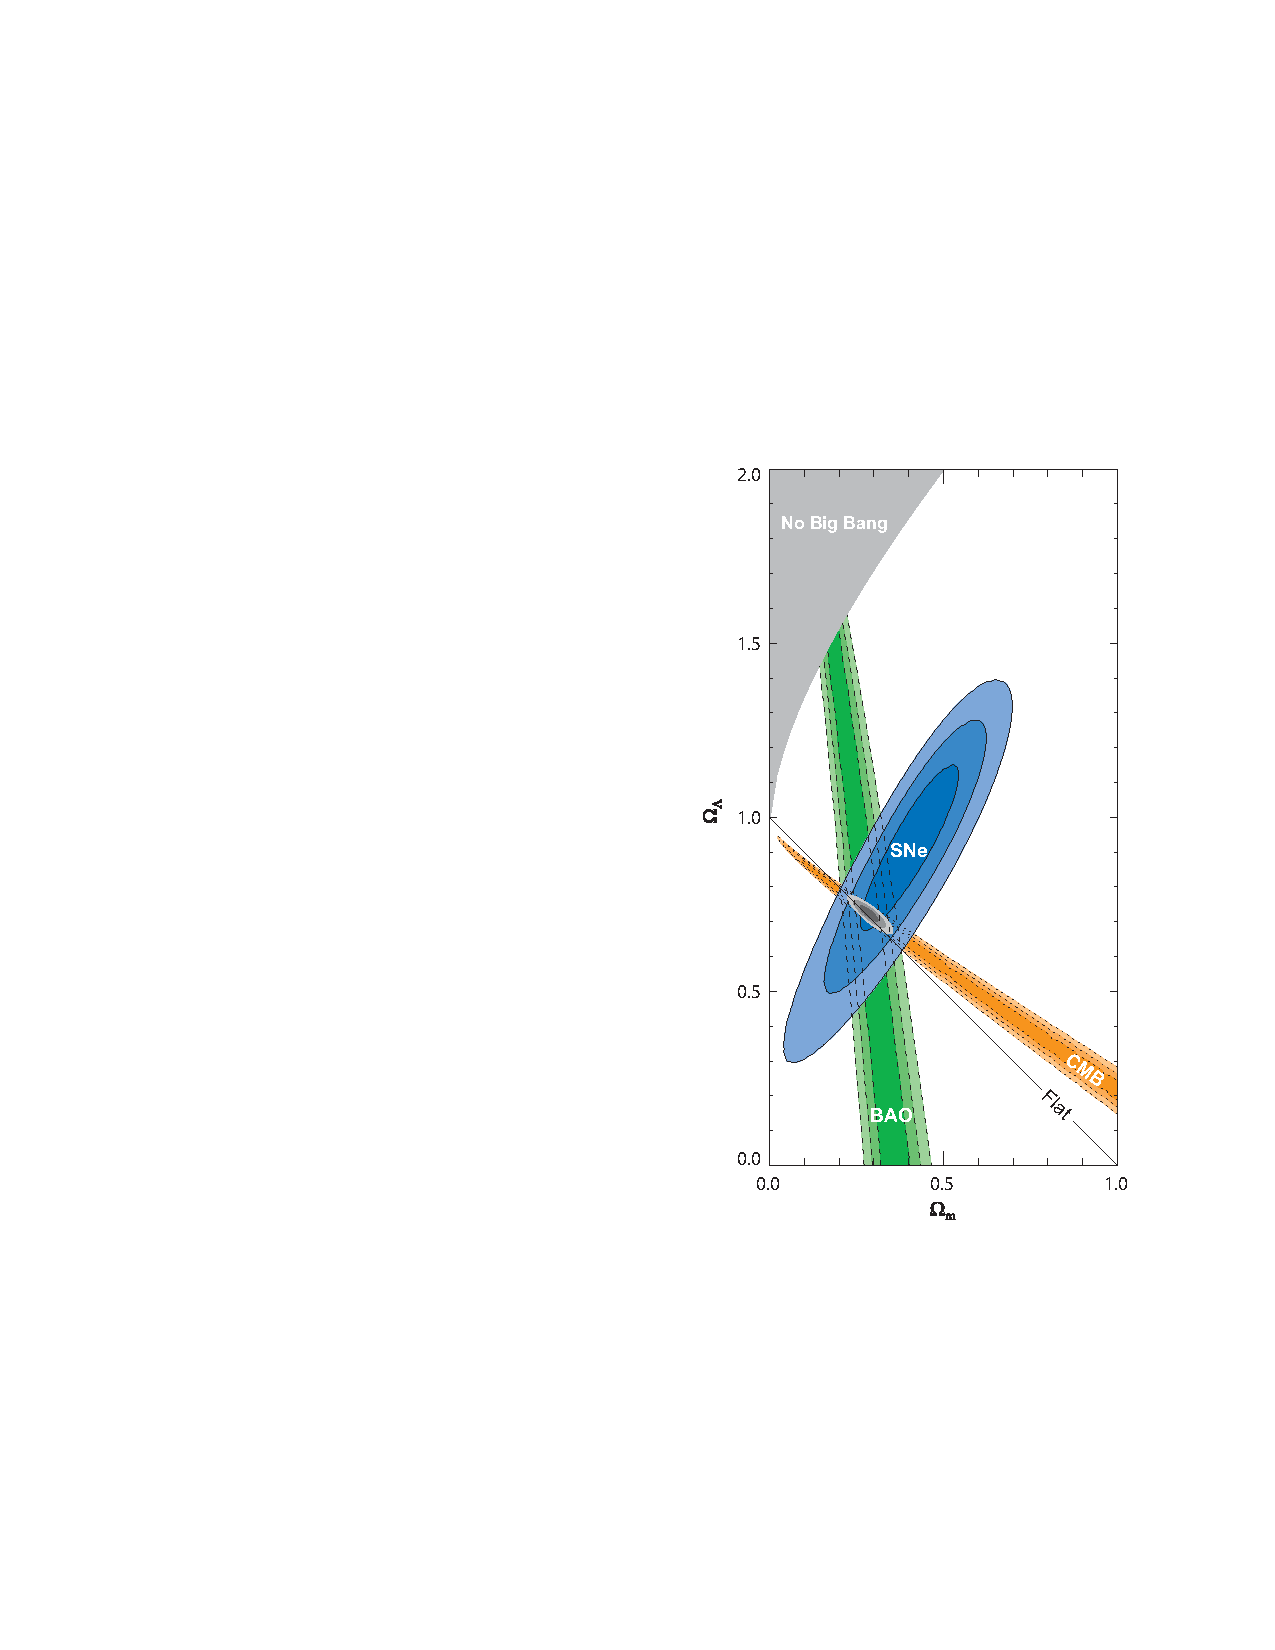
\includegraphics[width=0.52\linewidth, trim=5 0 0 0, clip=true]{lcdm1}\\
\hspace{5mm}\tiny{\color[rgb]{0, 0, 0}Kowalski et al \emph{ApJ} 2008}\\
\end{columns}

\begin{textblock}{32}(84,20)
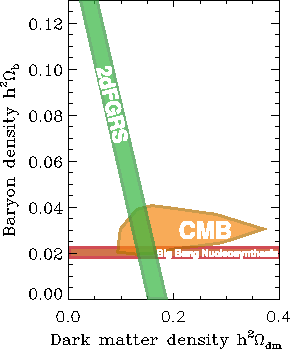
\includegraphics[width=\linewidth]{lcdm2}
\end{textblock}

\end{frame}

\begin{frame}
  \frametitle{But what about inflation?}
  
  \begin{exampleblock}{Question}
   Isn't inflation part of the $\Lambda$CDM model?
  \end{exampleblock} 

  \visible<2->{
  \begin{block}{Answer}
   Not really, no.
  \end{block}}

  \visible<3->{Approximately scale-invariant spectrum of perturbations to start with, on CMB scales (small wavenumber $k$)? \alert{Yes.}\\Due to inflation by definition? \alert{No.}
  \begin{equation}
  \mathcal{P}_\delta(k) \varpropto \mathcal{P}_\mathcal{R}(k) \varpropto k^{n_s - 1 \visible<4->{+\alpha\log k/k_0}}
  \end{equation}}
  \hspace{-1mm}\visible<5->{$\Lambda$CDM does not \textit{demand} inflation, just as it does not \textit{demand} any particular CDM\\\footnotesize
  \hspace{4mm}$-$inflation is just an idea for getting the required spectrum on CMB scales\\
  \hspace{4mm}$-$any particular DM model is just an idea for getting CDM}

\end{frame}

\section{Power spectra of cosmological perturbations}

\subsection{Background}

\begin{frame}
\frametitle{Generation of perturbations}

During inflation (or its alternative), quantum fluctuations seed energy/density perturbations
{\footnotesize
\bi
 \item on all length scales, e.g. 
 \begin{equation}
   \mathcal{P}_\delta(k) \varpropto k^{n_s - 1 \visible<2->{+\alpha\log k/k_0}}
 \end{equation}
 \visible<3->
 {
   \item with some distribution of amplitudes -- often assumed to be Gaussian:
   \begin{equation}
     \mathrm{pdf}(\delta) = \frac{1}{\sqrt{2\pi}\sigma^2_{\chi,H}(z_\mathrm{X},R)} \exp\left(-\frac{\delta^2}{2\sigma^2_{\chi,H}(z_\mathrm{X},R)^2}\right)
   \end{equation}
 }
\ei}

\visible<4->{Universe inflates $\rightarrow$ causes perturbations to exit the horizon (move out of causal contact with each other)\vspace{3mm}}

\visible<5->{Universe stops inflating, keeps expanding $\rightarrow$ catches up with the perturbations\vspace{3mm}}

\visible<6->{$\implies$ first out, last in (bigger-scale perturbations re-enter later)}

\end{frame}

\begin{frame}
\frametitle{Growth of perturbations}

Post-inflation, Universe quickly becomes \alert{radiation-dominated}
\begin{itemize}
  \item[\textcolor{black}{$\implies$}] baryons + photons coupled by electromagnetism\\
  \item[\textcolor{black}{$\implies$}] growth of perturbations damped by radiation free-streaming\\
  \item[\textcolor{black}{$\implies$}] growth of perturbations is \alert{logarithmic only}
\end{itemize}
\begin{equation}
\delta\varpropto\log R
\end{equation}

At $z\sim3000$, baryons kinetically decouple as Universe becomes \alert{matter-dominated}
\begin{itemize}
  \item[\textcolor{black}{$\implies$}] damping relieved\\
  \item[\textcolor{black}{$\implies$}] perturbations grow linearly, structure growth begins
\end{itemize}
\begin{equation}
\delta\varpropto R
\end{equation}

\end{frame}

\bfr{Observation of perturbations}

Essentially all cosmological observables depend on 2 things:
\begin{enumerate}
\item The initial spectrum of perturbations\\
   = distribution of amplitudes over scales: \mbox{\alert{$\mathsf{pdf}(\delta,k)$, $\mathcal{P}_\delta(k)$}}
   \bi \item[$\rightarrow$] this (mostly) comes from your theory of inflation \ei
\item How the perturbations + their consequences are processed \bi
  \item[$\rightarrow$] the geometry of the Universe over time: \alert{$H(t)$}
  \item[$\rightarrow$] the specific content of the Universe: \alert{$\mathcal{L}_\mathsf{SM+BSM}$} \bi
      \item[-] new particles 
      \item[-] exotic objects (e.g. cosmic strings)
      \item[-] specific processing events associated with the content\\(BBN, phase transitions, etc)
    \ei
  \ei
\end{enumerate}

$\implies$ can use CMB, large scale structure, etc to test specific particle theories\\
(\alert{not} just how much stuff with each $w$ and its impact on $H(t)$)

\end{frame}

\subsection{Middle Universe observables}

\bfr{The cosmic microwave background (CMB)}
Key is to look at amount of power on different scales for info on primordial spectrum and processing physics\vspace{6mm}

  \begin{columns}[t]
  \column{0.65\textwidth}
    \centering\tiny Planck Paper XV
    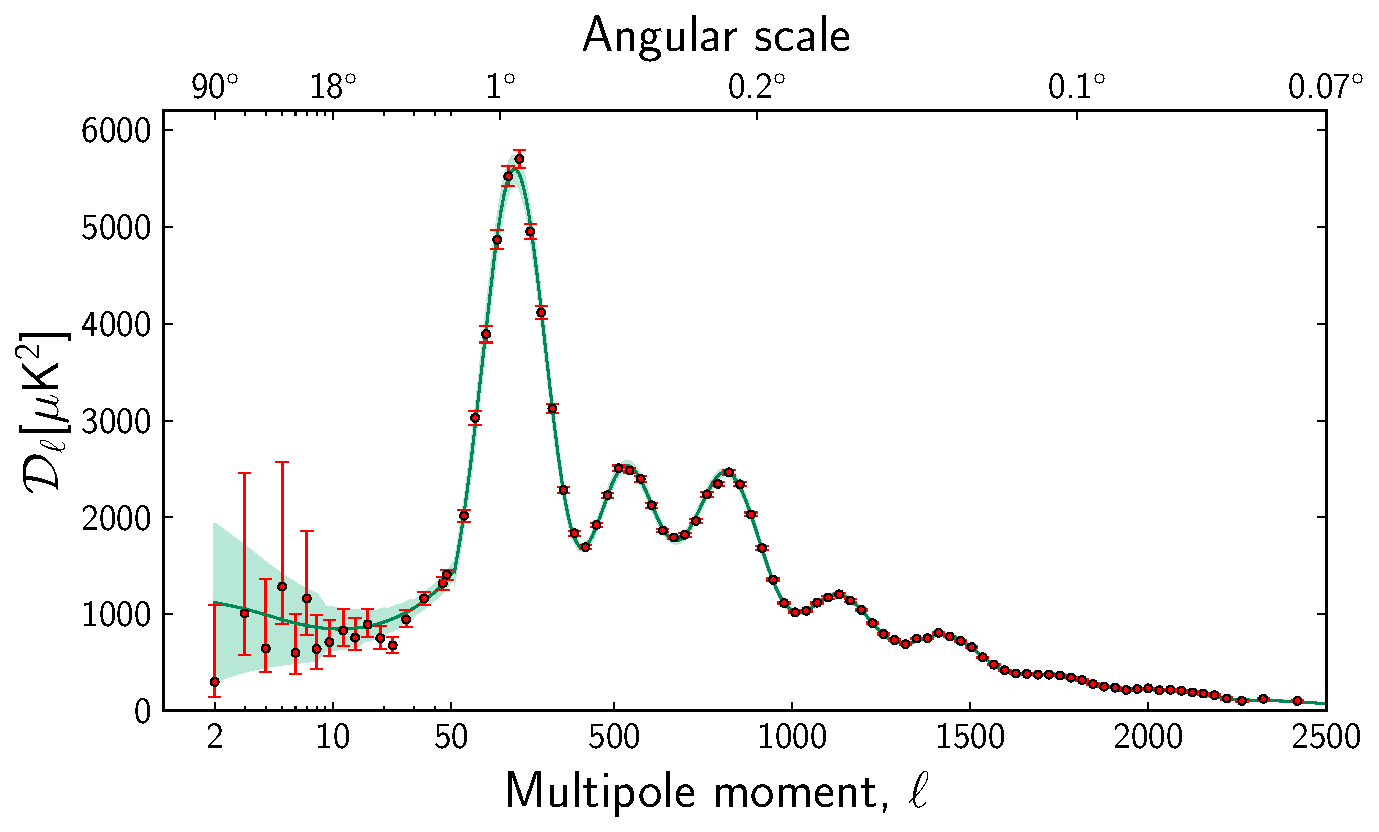
\includegraphics[width=\columnwidth]{cmbtot_loglin}
  \column{0.6\textwidth}
    \centering\tiny Hunt \& Sarkar (\textit{JCAP} 2014)
    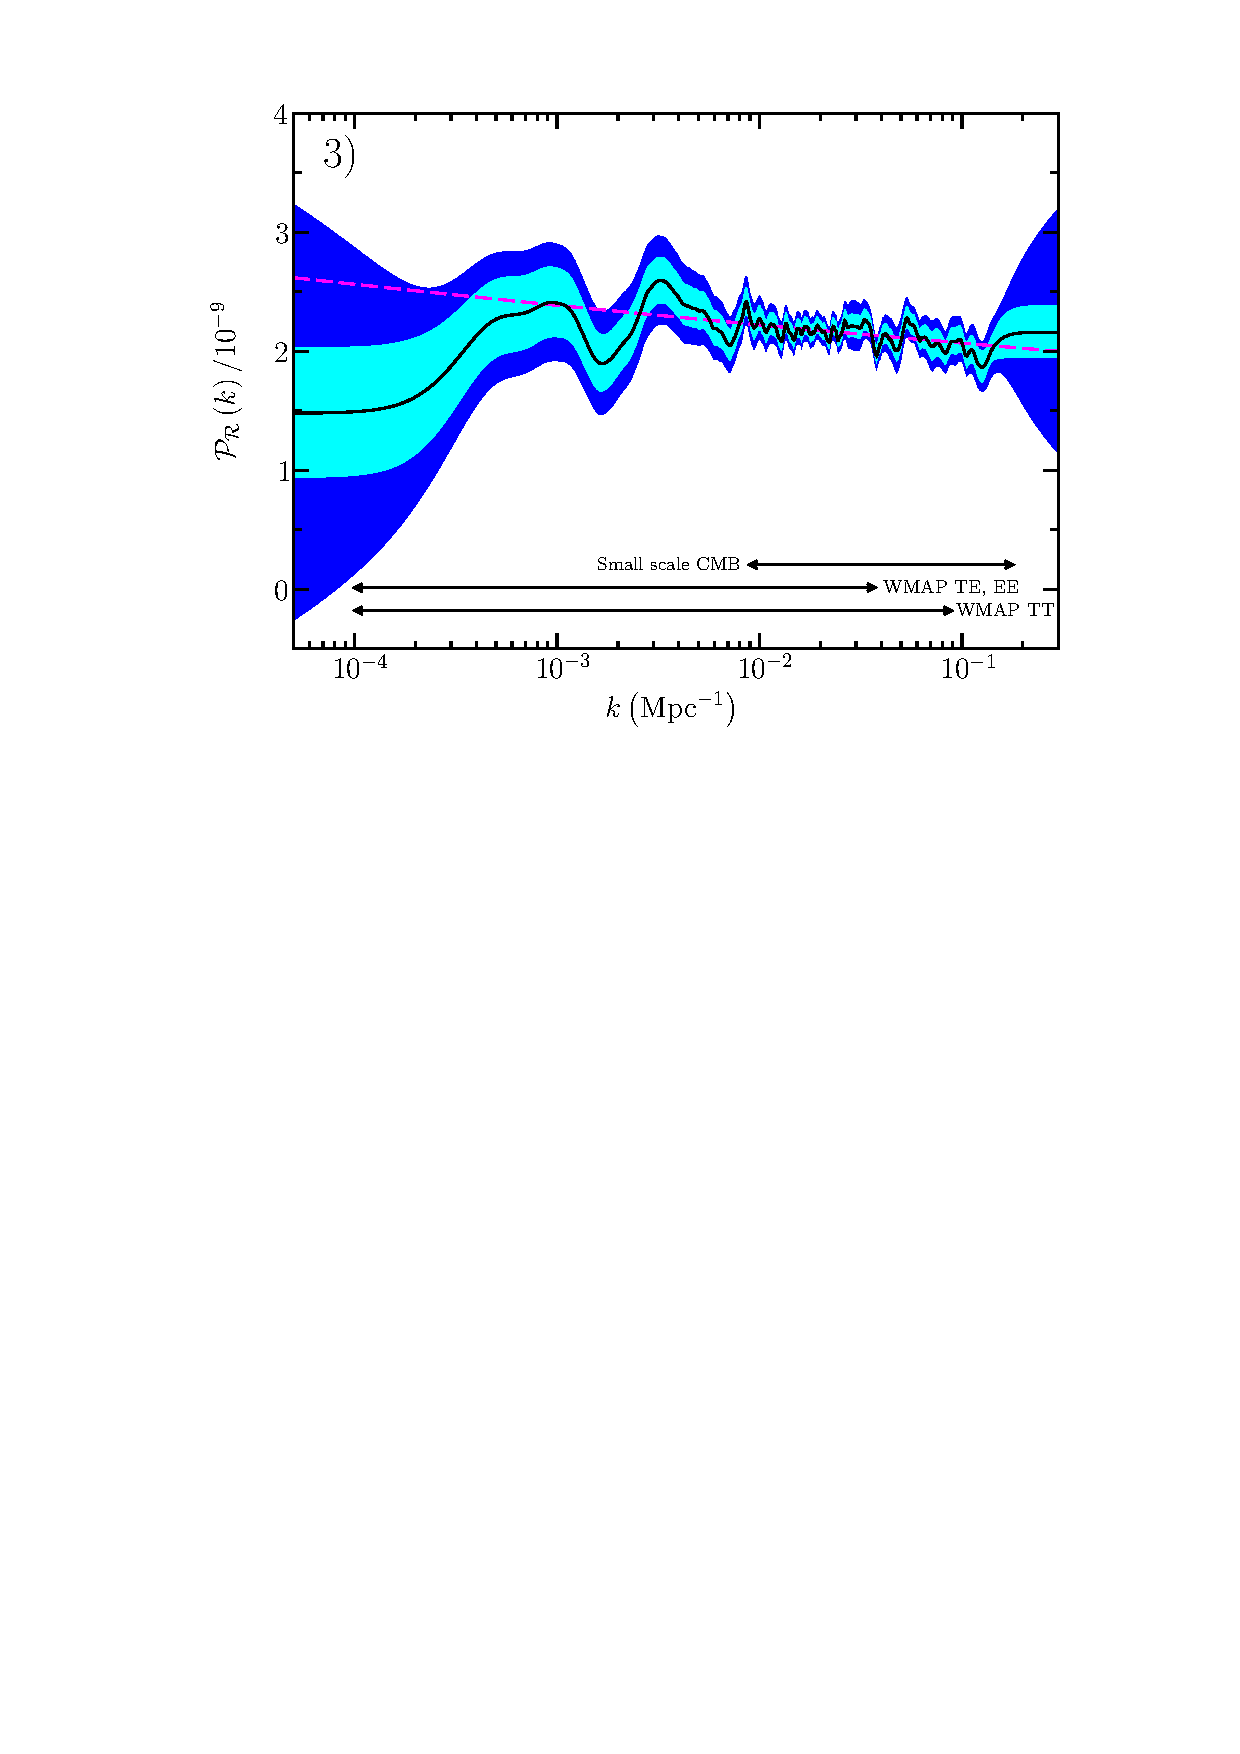
\includegraphics[width=\columnwidth, trim = 60 0 0 0, clip=true]{fig18c}
  \end{columns}

\end{frame}

\bfr{The CMB -- inflation-like examples}

  \begin{columns}
  \column{0.65\textwidth}
    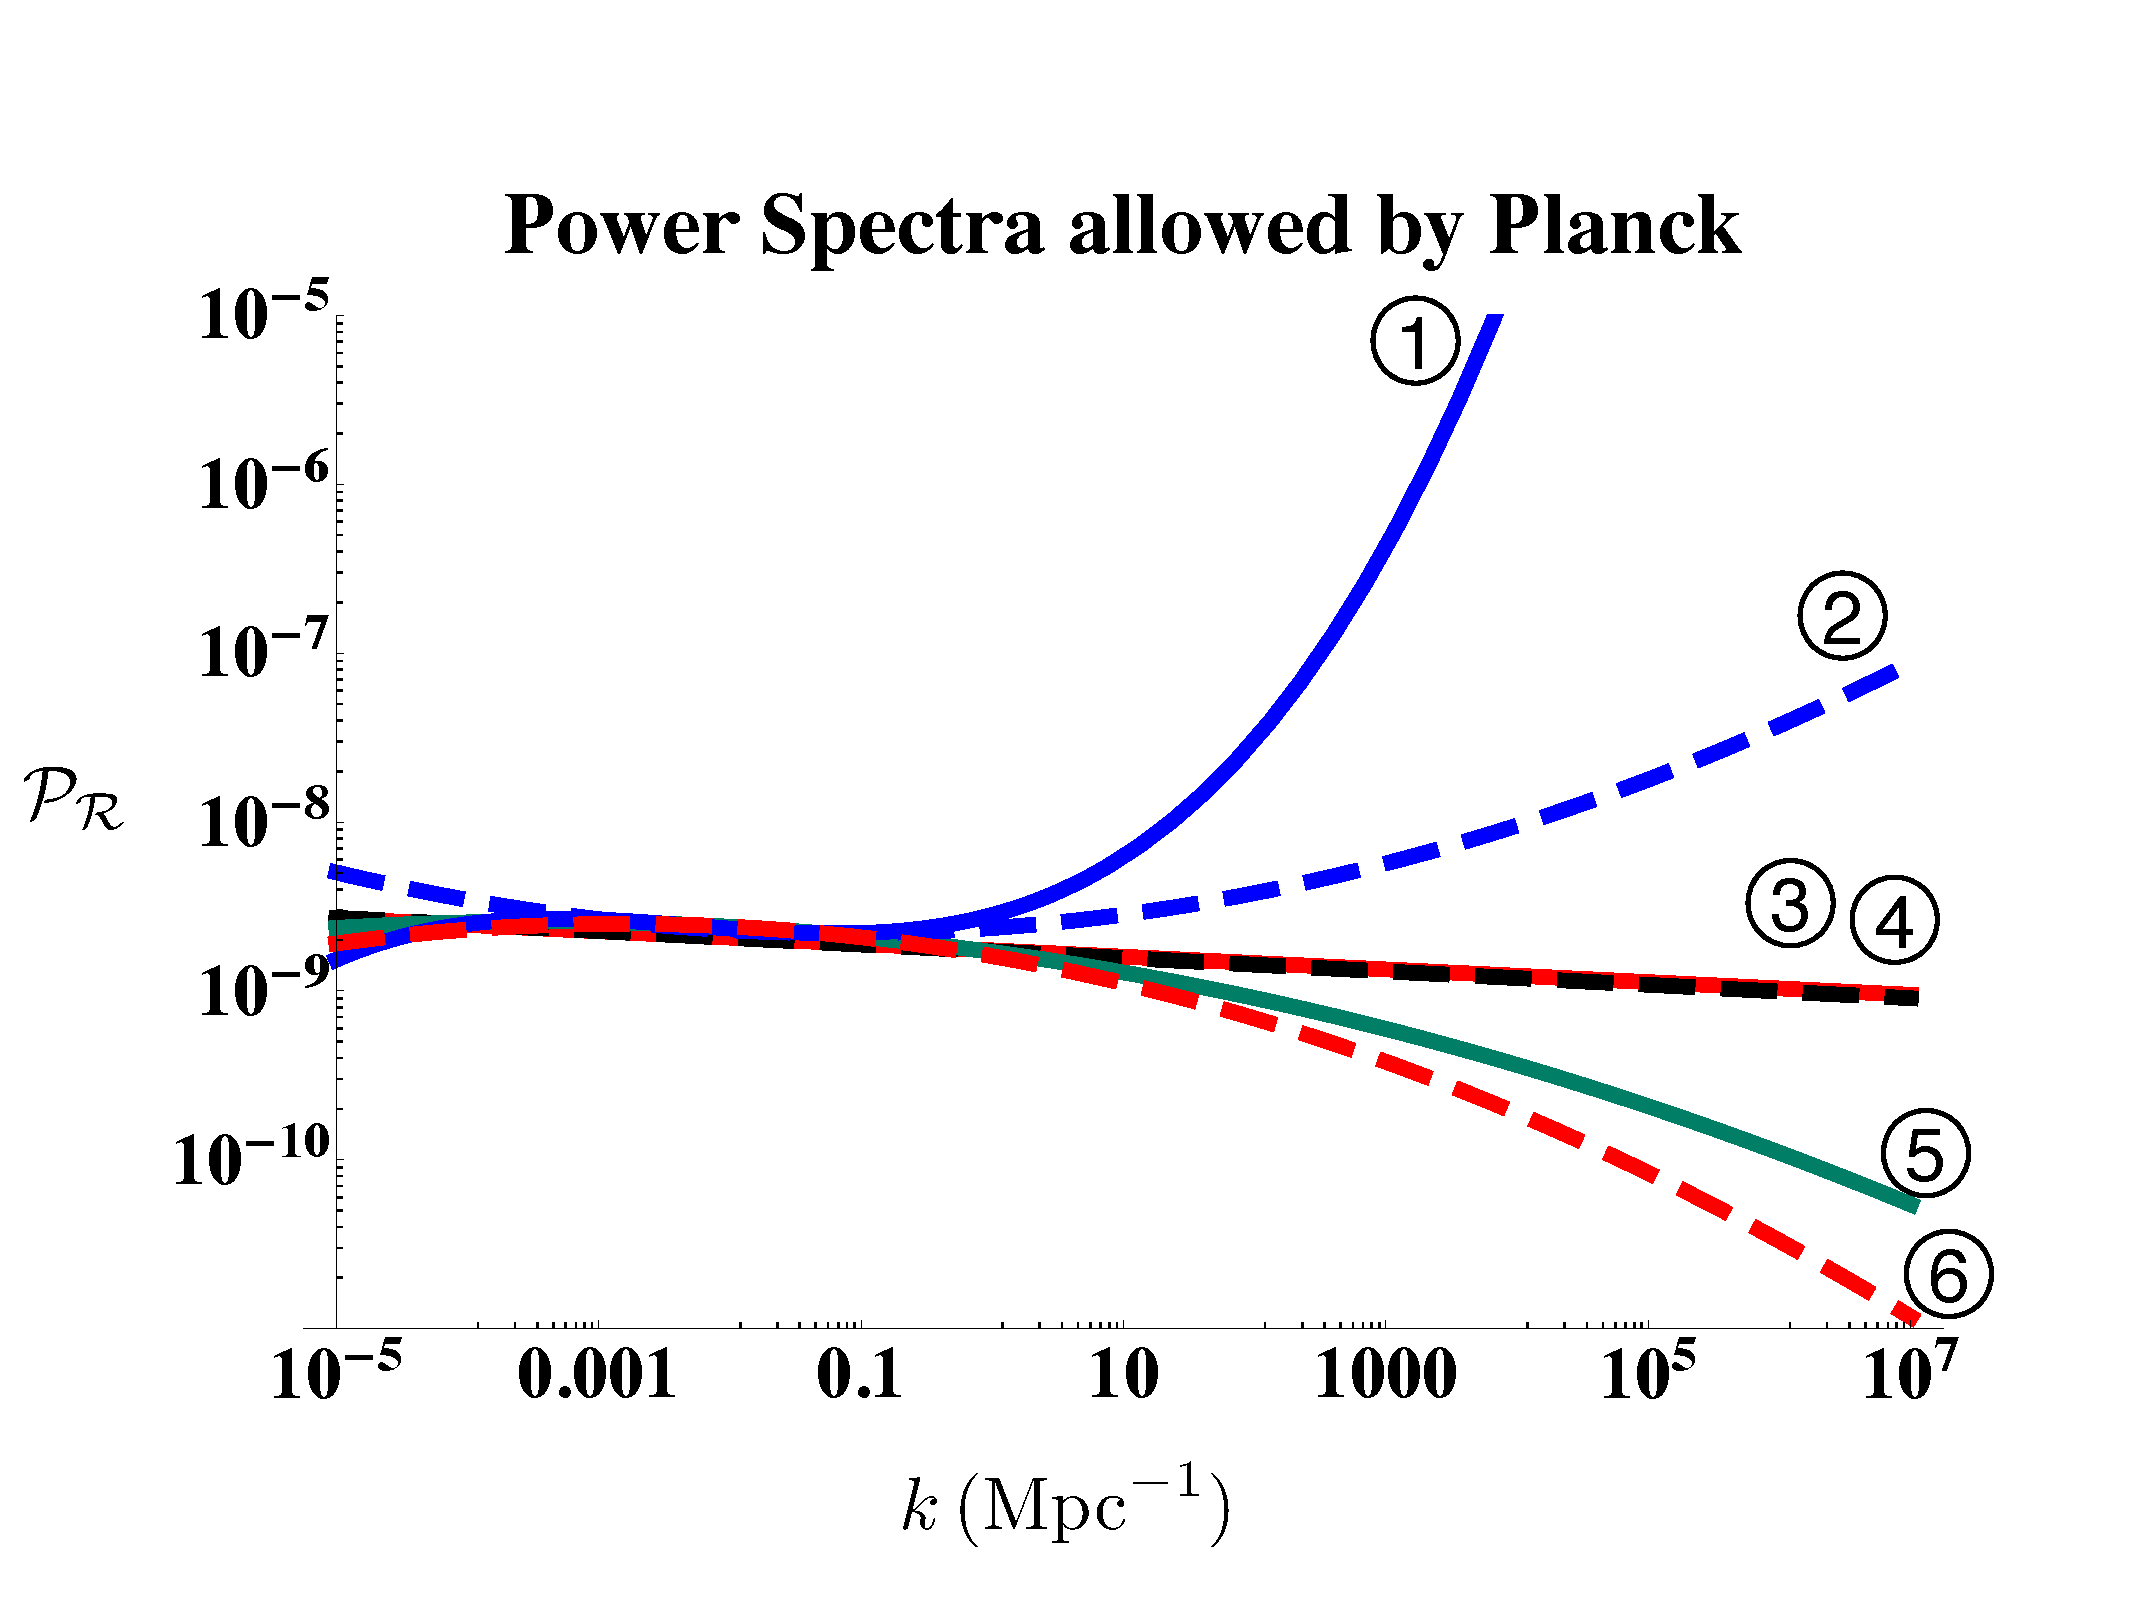
\includegraphics[width=\columnwidth, trim = 60 0 0 0, clip=true]{PlanckPSThickAxes}
  \column{0.55\textwidth}
    \footnotesize
    \begin{enumerate}
      \item $\Lambda$CDM + $dn_s/d{\rm ln}k$ + $d^2(n_s)/d{\rm ln}k^2$, {\it Planck}+WMAP polarisation (WP)
      \item $\Lambda$CDM + $r$ + $dn_s/d{\rm ln}k$, {\it Planck}+WP
      \item $\Lambda$CDM + $r$, {\it Planck}+WP
      \item $\Lambda$CDM, {\it Planck}+WP
      \item $\Lambda$CDM + $dn_s/d{\rm ln}k$, {\it Planck}+WP
      \item $\Lambda$CDM + $r$ + $dn_s/d{\rm ln}k$, {\it Planck}+WP+BAO
    \end{enumerate}
  \end{columns}

  \begin{textblock}{60}(30,80)
    \tiny Shandera, Erickcek, PS \& Yana Galarza \emph{Phys.\ Rev.\ D} 2013
  \end{textblock}

\end{frame}


\bfr{Large scale structure (LSS)}
\footnotesize
\bi
  \item Density perturbations $\equiv$ sound waves $\rightarrow$ matter density oscillations
  \item Seen in CMB temperature, polarisation anisotropy at $z\sim1100$\\\vspace{1mm}
  \item Eventually grow to form galaxies, etc at $z\lesssim20$
\ei

  \begin{columns}[c]
  \column{0.55\textwidth}
    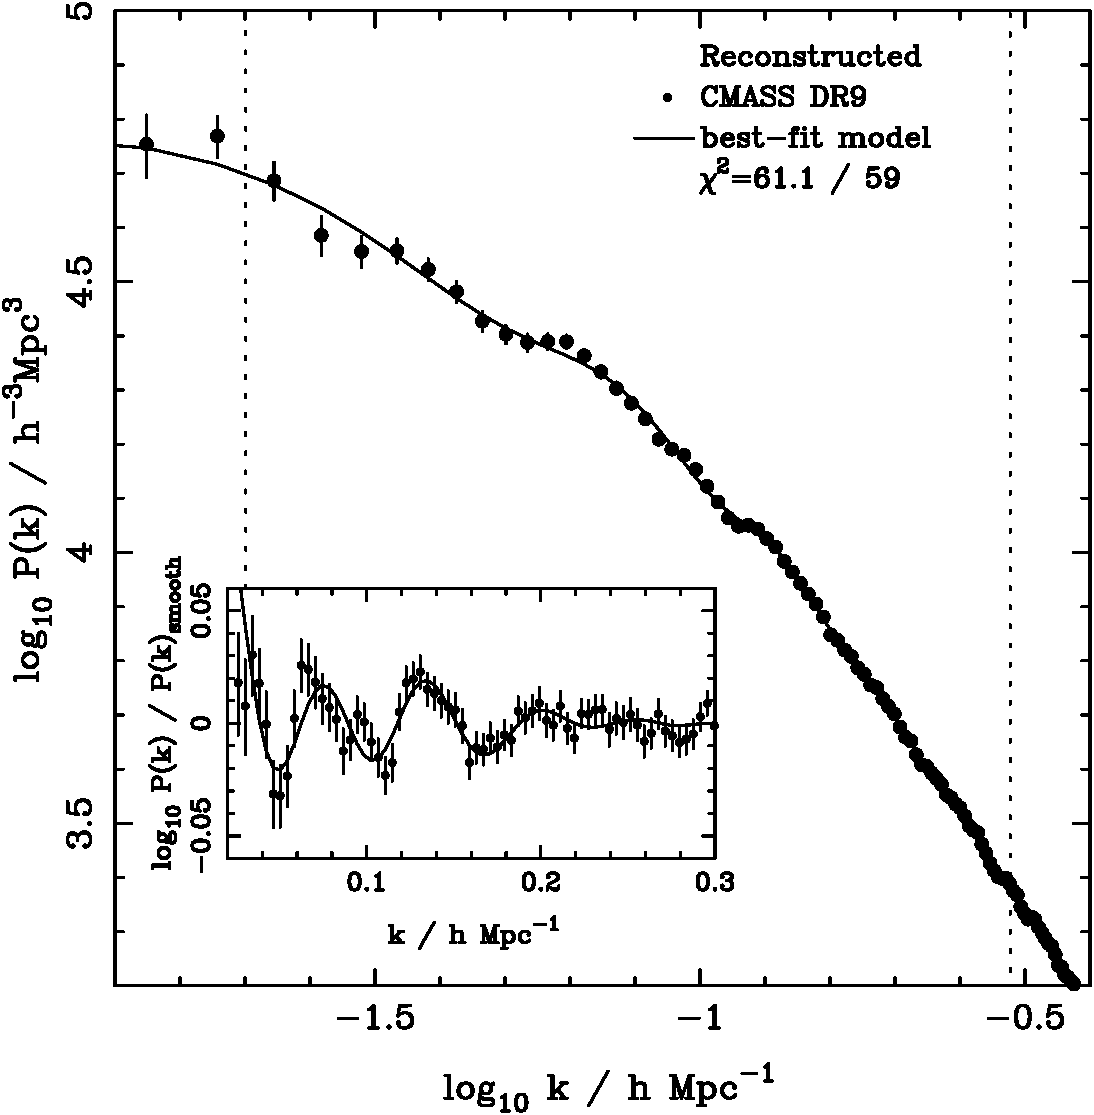
\includegraphics[width=0.85\columnwidth, trim = 0 0 0 0, clip=true]{BOSS_DR9_Pk_recon}
  \column{0.55\textwidth}
    Some imprint of scales of density oscillations (=primordial spectrum) retained $\rightarrow$ \alert{Baryon Acoustic Oscillations}\vspace{3cm}
  \end{columns}

\begin{textblock}{40}(70,70)
  {\tiny SDSS-III Data Release 9 \emph{MNRAS} 2012}
\end{textblock}

\end{frame}


\bfr{Large scale structure -- neutrino mass example}

\footnotesize
Neutrinos are warm dark matter
\bi
\item[$\implies$] large free-streaming length, depends on $m_\nu$ \\$\rightarrow$ escape from small collapsing perturbations
\item[$\implies$] Suppression in small-scale matter (processed) power spectrum
\ei

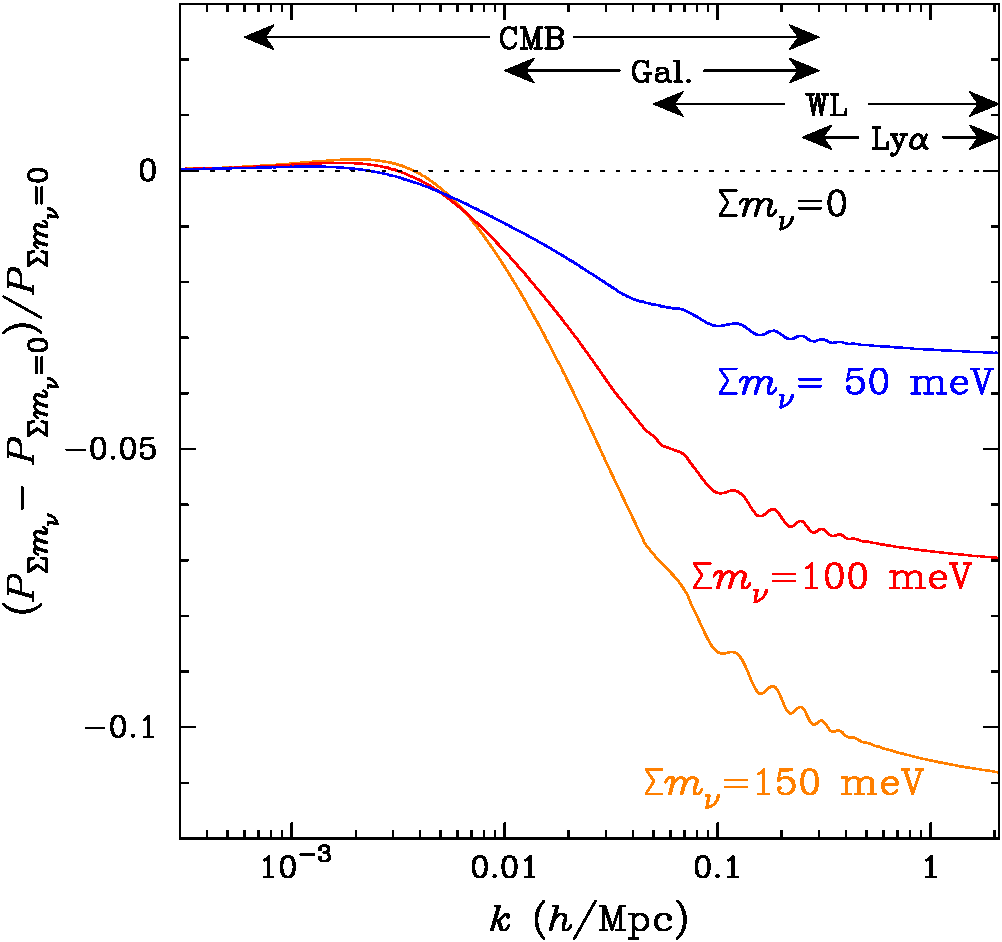
\includegraphics[width=0.55\columnwidth, trim = 0 0 0 0, clip=true]{relative_pk}

\begin{textblock}{40}(75,75)
  {\tiny SNOWMASS 2013, arXiv:1309.5383}
\end{textblock}

\end{frame}


\subsection{Rare objects}

\bfr{Rare objects: primordial black holes (PBHs)}

  \begin{exampleblock}{Question}
     What is a \textit{primordial} black hole?
  \end{exampleblock}
  \bi
    \item If density perturbations are big enough ($\delta>0.3$), when they enter the horizon the whole thing collapses\\ 
          $\rightarrow$ immediate black hole
    \item PBH mass is horizon mass at re-entry
    \item[$\implies$] number of PBHs with $M_\mathsf{PBH}$ maps directly to amplitude of perturbations on some scale $k$
  \ei

  \bi
    \item For some distribution of perturbations $\mathrm{pdf}(\delta)$
    \footnotesize
    \begin{equation}
      \label{relicdens}
      \beta_{\mathrm{PBH}} \equiv \Omega_{\mathrm{PBH}} / \Omega_0 = \int^{\infty}_{\delta_\mathrm{min}} \mathrm{pdf}(\delta)\,\mathrm{d}\delta
    \end{equation}
  \ei

  Can repeat at different $k$ to get limits on primordial spectrum\\
  $\rightarrow$ limits on inflationary theories

\end{frame}


\bfr{Rare objects: ultracompact minihalos (UCMHs)}

  \begin{exampleblock}{Question}
  What is an \textit{ultracompact} minihalo (UCMH)?
  \end{exampleblock} 

  \visible<2->{
  \begin{block}{Answer}
  A DM halo that collapses shortly after matter-radiation equality\\
  $\implies$ from a large amplitude density perturbation 
  \end{block}}
  
  \footnotesize
  \visible<3->{
    \begin{itemize}
      \item[]`Shortly' means $z_\mathrm{collapse}$ is ${O}(100)$ or more \vspace{2mm}
      \item[]\hspace{3mm}$\implies$ isolated collapse \vspace{2mm}
      \item[]\hspace{3mm}$\implies$ formation by radial infall \vspace{2mm}
      \item[]\hspace{3mm}$\implies$ very steep density profile $\rightarrow \rho\varpropto r^{-9/4}$ \vspace{2mm}
      \item[]\hspace{3mm}$\implies$\alert{excellent indirect detection targets} \vspace{2mm}
      \item[]Also good lensing prospects {\tiny Ricotti \& Gould \emph{ApJ} 2009; Li et al \emph{Phys.~Rev.~D} 2012}
    \end{itemize}
  }

  \begin{textblock}{28}(83,73)
  \visible<3>{\tiny PS \& Sivertsson \\ \emph{Phys.\ Rev.\ Lett.} 2009\\ Lacki \& Beacom \emph{ApJL} 2010}
  \end{textblock}

\end{frame}


\begin{frame}
  \frametitle{Rare objects: UCMH formation}

    \textbf{Conditions for formation}
    \begin{itemize}
      \item{Seeded well before matter-radiation equality}\vspace{1mm}
      \item{Requires $\delta \gtrsim \mathcal{O}(10^{-3})$}\\(compare with normal inflationary perturbations $\delta \sim 10^{-5}$)\vspace{1mm}
      \item{$\longrightarrow$ much more likely than PBH formation ($\delta \gtrsim 0.3$)}\vspace{1mm}
    \end{itemize} 

    \textbf{Usefulness}
    \begin{itemize}
      \item{Like PBHs, UCMH mass set by horizon scale at time of horizon entry}\vspace{1mm}
      \item{$\implies$ specific UCMH mass $\equiv$ specific cosmological scale}\vspace{1mm}
      \item{$\implies$ limit on abundance of specific mass halo $\equiv$ limit on power on specific scale $k$}
    \end{itemize}

\end{frame}


\bfr{Rare objects: observational limits}

  \bi
    \item[\textbf{PBHs}:] energetic particles from evaporation, lensing, binary disruption
    \item[\textbf{UCMHs}:] energetic particles from DM annihilation, lensing
  \ei

  \begin{columns}
  \column{0.6\textwidth}
    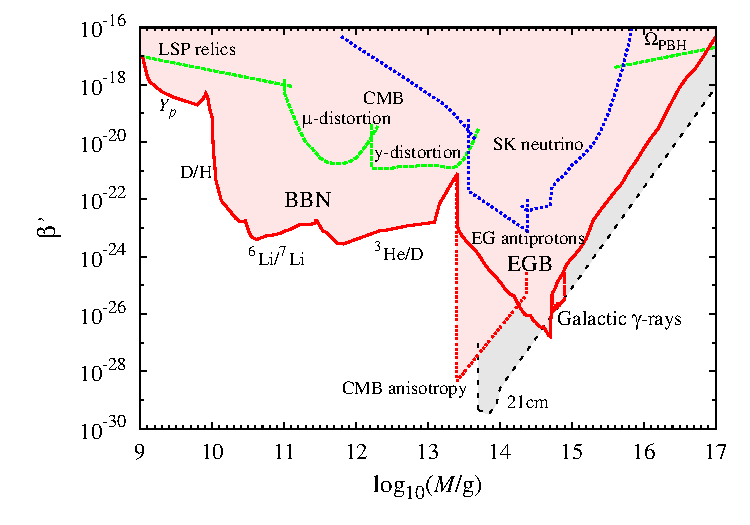
\includegraphics[width=\columnwidth]{combined}
  \column{0.5\textwidth}
    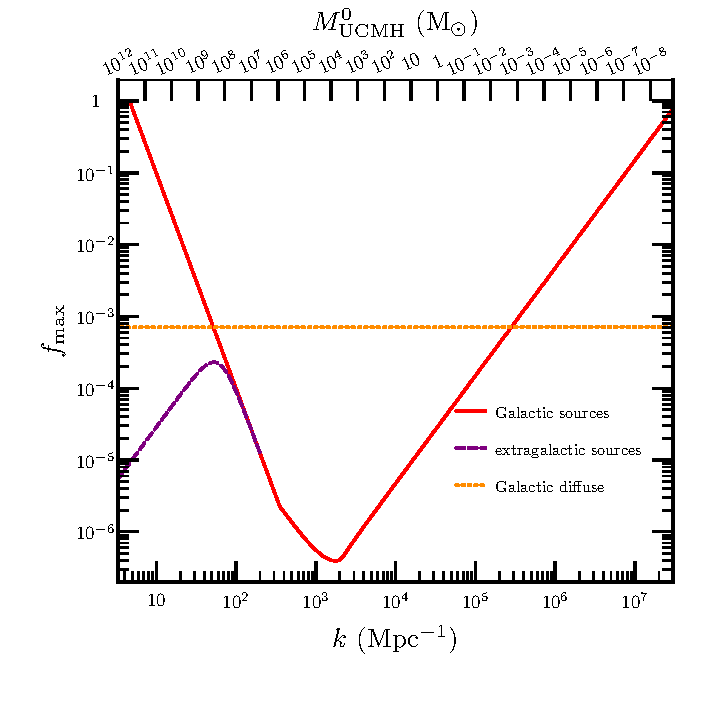
\includegraphics[width=\columnwidth]{Fig1}
  \end{columns}
 
  \begin{textblock}{40}(70,82)
    {\tiny Bringmann, PS \& Akrami, \emph{Phys.~Rev.~D} 2012}
  \end{textblock}

  \begin{textblock}{40}(20,80)
    {\tiny Josan et al, \emph{Phys.~Rev.~D} 2009\\\vspace{-2mm}
           Carr et al, \emph{Phys.~Rev.~D} 2010}
  \end{textblock}

\end{frame}


\begin{frame}
  \frametitle{Rare objects: comparative limits on power spectrum}

  \vspace{5mm}
  Limits on $\mathcal{P}_\delta$ from UCMHs $\sim$5 orders better than from PBHs\\
  $\implies$ strong limits on inflationary models

  \vspace{-30mm}
  \begin{columns}
  \column{\textwidth}
    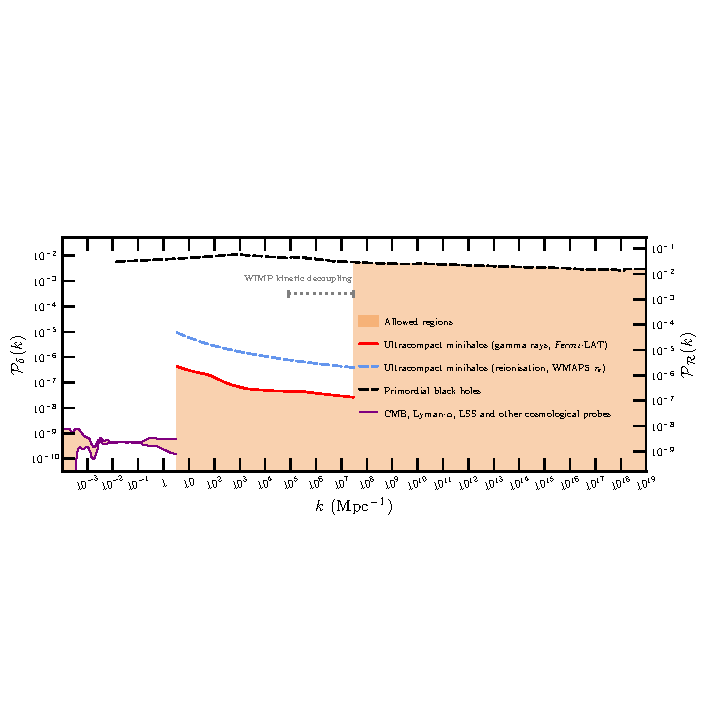
\includegraphics[width=\columnwidth]{Fig6}
  \end{columns}

\begin{textblock}{40}(70,80)
{\tiny Bringmann, PS \& Akrami, \emph{Phys.~Rev.~D} 2012}
\end{textblock}

\end{frame}


\begin{frame}
  \frametitle{Implications for inflation -- slow-roll reconstruction}

  \begin{columns}
  \column{0.53\textwidth}
    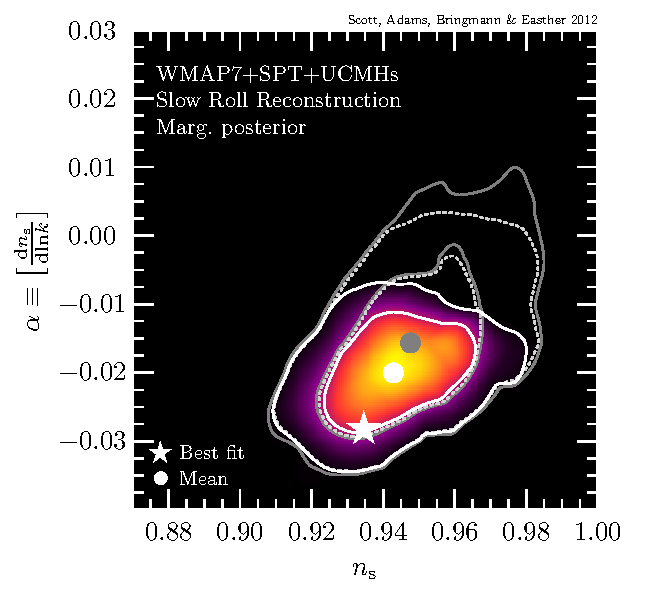
\includegraphics[height=0.9\columnwidth]{slowroll1}
  \column{0.53\textwidth}
    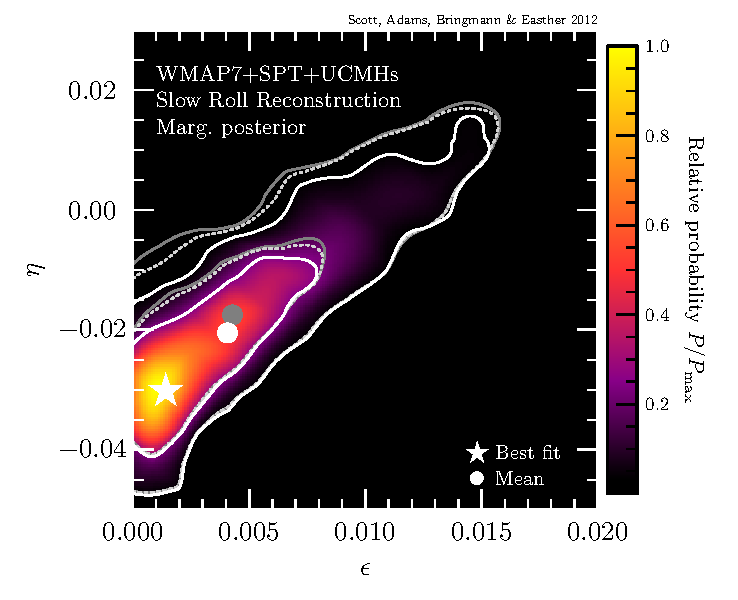
\includegraphics[height=0.9\columnwidth]{slowroll2}
  \end{columns}

  Impacts on slow-roll reconstruction

  grey: original\hspace{5mm} dashed: $z_\mathrm{c}=200$\hspace{5mm} colours: $z_\mathrm{c}=50$
  
  (but beware extrapolation of $\alpha$ from WMAP scales)

\end{frame}


\section[Specific particle/field processes]{Specific particle/field processes \bf (optional)}


\subsection{BBN}

\bfr{Big Bang Nucleosynthesis (BBN)}

  \begin{columns}
  \column{0.53\textwidth}
    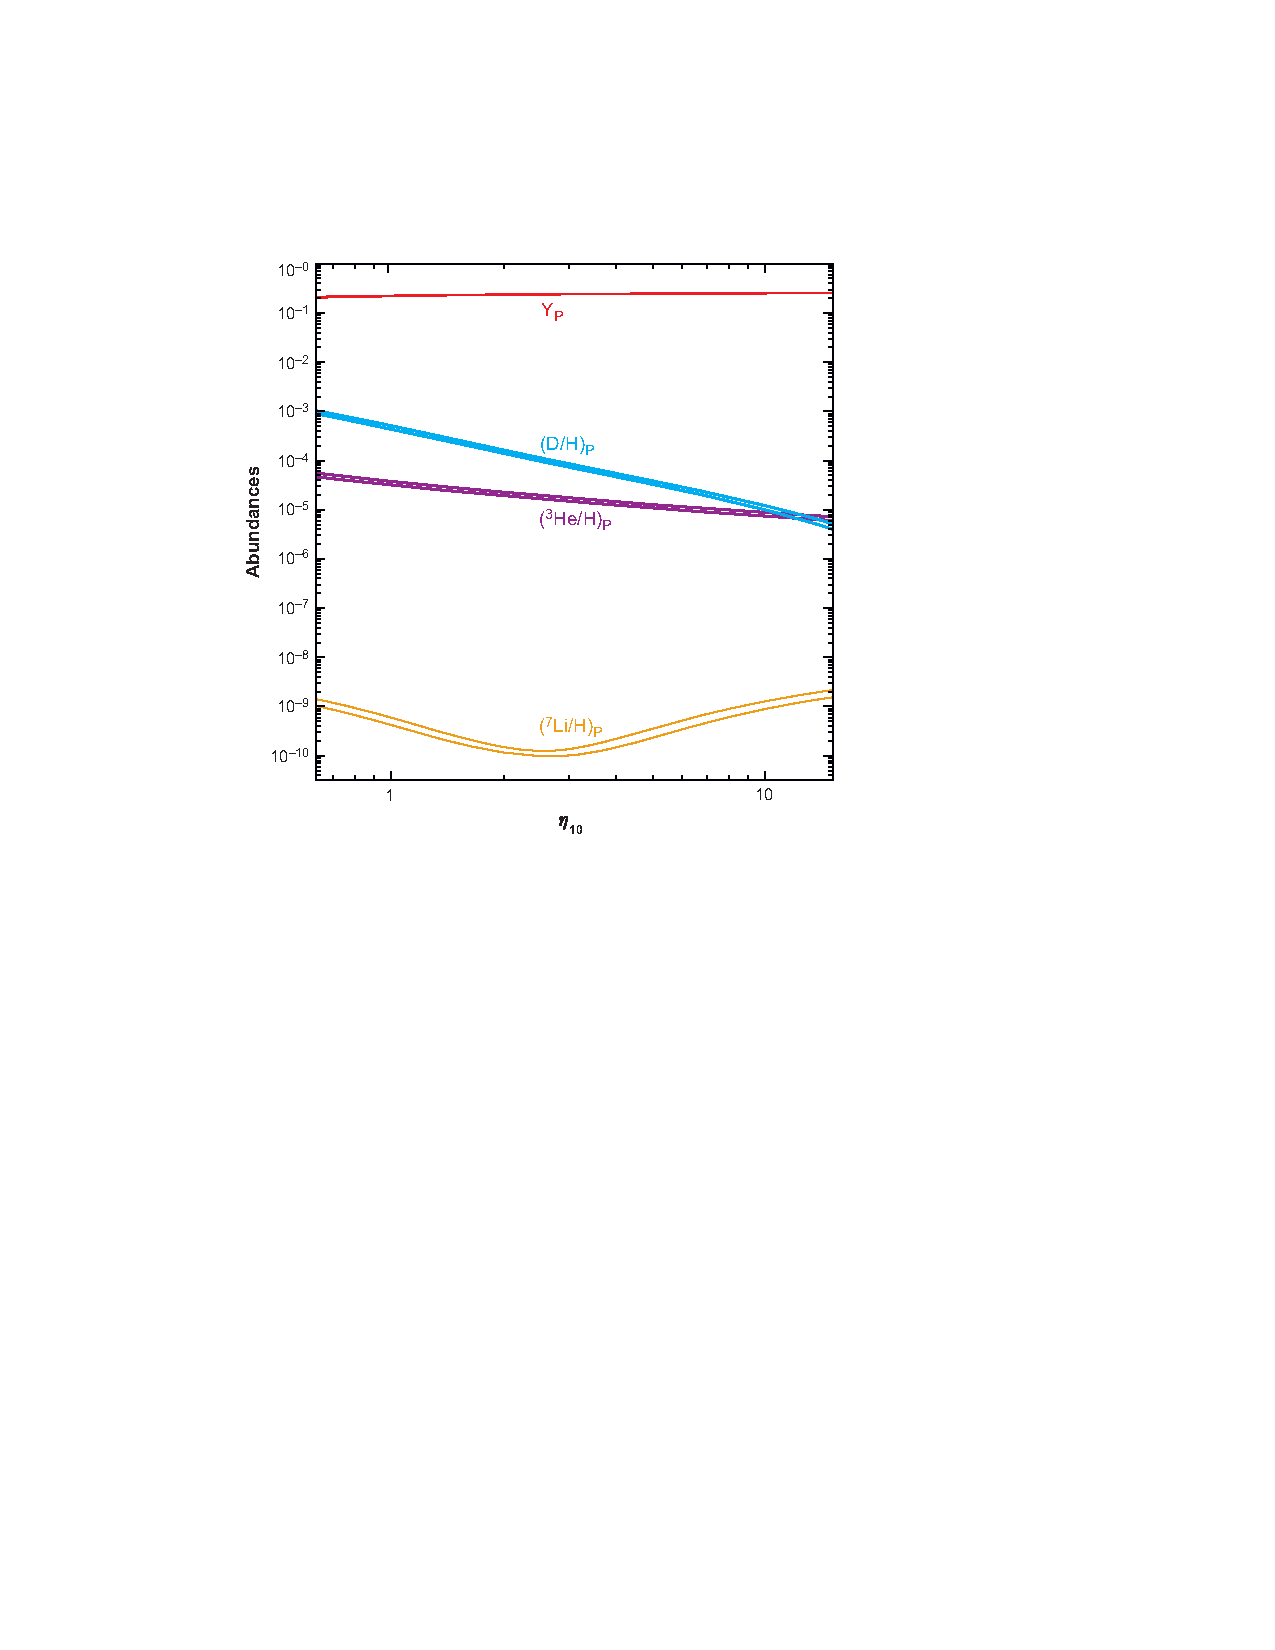
\includegraphics[height=0.9\columnwidth]{bbn}
  \column{0.53\textwidth}
    \bi
      \item Light elements (H, He, Li, B, Be) form when Universe cools to $T \sim$ a few MeV
      \item Relative amounts are sensitive to baryon-to-photon ratio $\eta$\\
            $\implies$ sensitive to $\Omega_\mathrm{b}$
      \item Can be messed up by additional energy injection from e.g.\bi
        \footnotesize
        \item Late-decaying or annihilating particles
        \item Evaporation of PBHs
      \ei
      \item[$\implies$] stringent bounds on new physics 
    \ei
  \end{columns}

\begin{textblock}{40}(20,76)
  {\tiny Iocco et al (\emph{Phys.~Repts.} 2009)}
\end{textblock}

\end{frame}


\subsection{Cosmic strings}

\bfr{Cosmic strings}

  \footnotesize
  \begin{columns}
  \column{0.8\textwidth}
    \bi
      \item Nothing (necessarily) to do with string theory
      \item 1D topological defect caused by field transition to different vacua in causally disconnected regions  
      \item Breaking of \textit{any} $U(1)$ symmetry in the early Universe should produce cosmic strings
      \item Searches for presence of strings can constrain particle theories up the the GUT scale
      \item Crucial quantity is string tension\\$G\mu$ $\varpropto$ symmetry-breaking scale$^2$
      \item Observational limits from\bi\footnotesize
        \item[-] CMB position-space maps
        \item[-] 21\,cm maps
        \item[-] pulsar timing
        \item[-] UCMH searches
      \ei
    \ei
  \column{0.3\textwidth}
    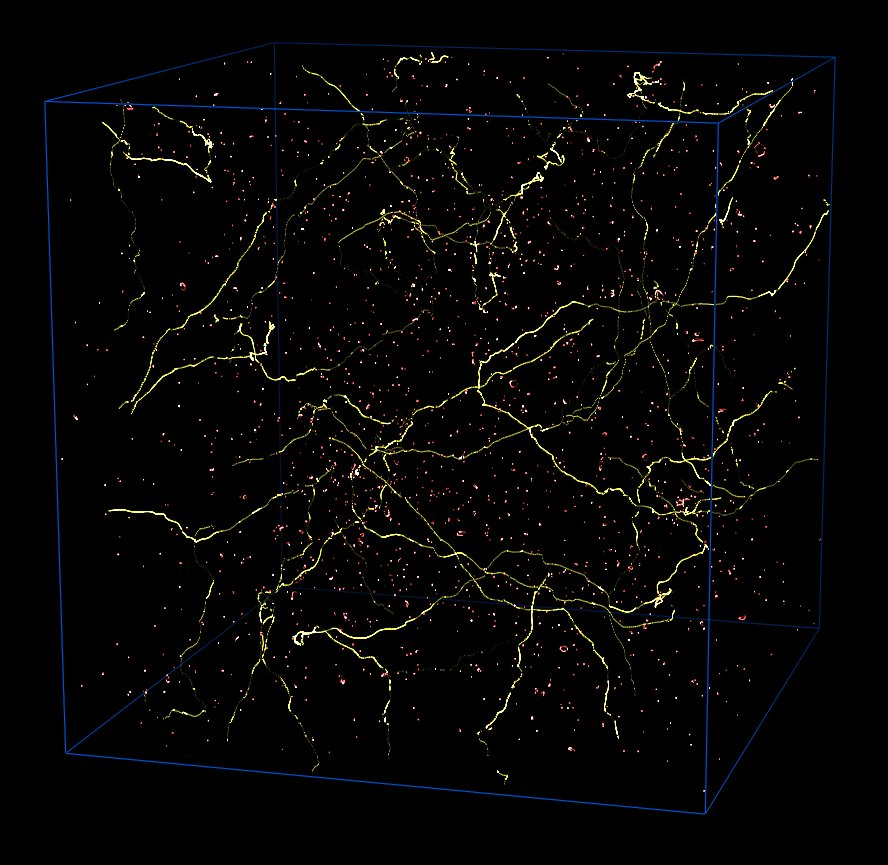
\includegraphics[width=\columnwidth]{cs_mat}\vspace{30mm}
  \end{columns}

\end{frame}


\subsection{Phase transitions and reheating}

\bfr{Phase transitions and reheating}

\footnotesize
\bi
\item As universe cools, vacuum goes through various phase transitions as symmetries break
  \bi
  \footnotesize
    \item Electroweak phase transition $\mathcal{O}(200\,\mathsf{GeV})$
    \item QCD/chiral symmetry breaking $\mathcal{O}(200\,\mathsf{MeV})$
    \item Breaking of symmetries associated with new physics
  \ei
\item Phase transitions may or may not produce:
  \bi
  \footnotesize
    \item defects like cosmic strings (depends on groups involved)
    \item strong density perturbations at a particular $k$ (depends on order of transition)
    \item impacts on concurrent processes like kinetic decoupling of dark matter (more tomorrow)
  \ei
\item Drastic changes in field content have similar character
  \bi
  \footnotesize
    \item Reheating: mass in inflaton field at end of inflation converted into other particles, heating Universe
    \item Particle genesis (baryo/lepto), creating matter asymmetry
  \ei
\ei

\end{frame}




\bfr{Take-home points}
\bi
  \item Cosmological observables are sensitive to

  \bi
    \item Initial distribution of density perturbations 
    \item Content of the Universe
  \ei
  \item[\textcolor{black}{$\implies$}] they can be used to test
  \bi
    \item Theories for inflation
    \item Theories for new symmetries + particles beyond the Standard Model
  \ei
  \item Inflation has few other observables to correlate this with
  \item \dots but many concrete Beyond Standard Model theories lead to correlated signals elsewhere $\rightarrow$ next 2 lectures 
\ei
\end{frame}

\end{document}

